
\documentclass[a4paper, french, 12pt]{article}


\usepackage[main=english,french]{babel}
\usepackage{arabtex}
\usepackage{utf8}
\setcode{utf8}
\usepackage[T1]{fontenc}
\usepackage[a4paper, margin=1in]{geometry}
\usepackage{fancyhdr}
\usepackage{graphicx}
\usepackage{amsmath,amssymb}


\renewcommand{\familydefault}{\sfdefault}


\pagestyle{plain}


\fancyhf{}
\lhead
{
    Université Sétif 1 \\
    Faculté des Sciences \\
    Département d'Informatique
}
\rhead
{
    2\textsuperscript{-ième} année(année 2023/24)\\
    Architecture des Ordinateurs\\
    Enseignant Kara Abdelaziz%
}
\cfoot{\thepage}


\title{\centering \textbf{Side-project: Cache memory}}
\author{}
\date{}





\begin{document}


%\setlength{\headheight}{80pt}
\maketitle
\thispagestyle{fancy}

\section{Preamble}

The project concerns the implementation of a memory cache interacting with its main memory, like depicted in the schematic below. We can see that it represents only the memory part of an 32 bits architecture without the processor. Essentially, a cache of 32 KBytes and a main memory of 64 MBytes of capacity. Normally the cache controller should be put apart from the cache memory, usually integrated to a component called the MMU (Memory Management Unit) within the CPU packaging, but in our implementation we will put them together in the same component.

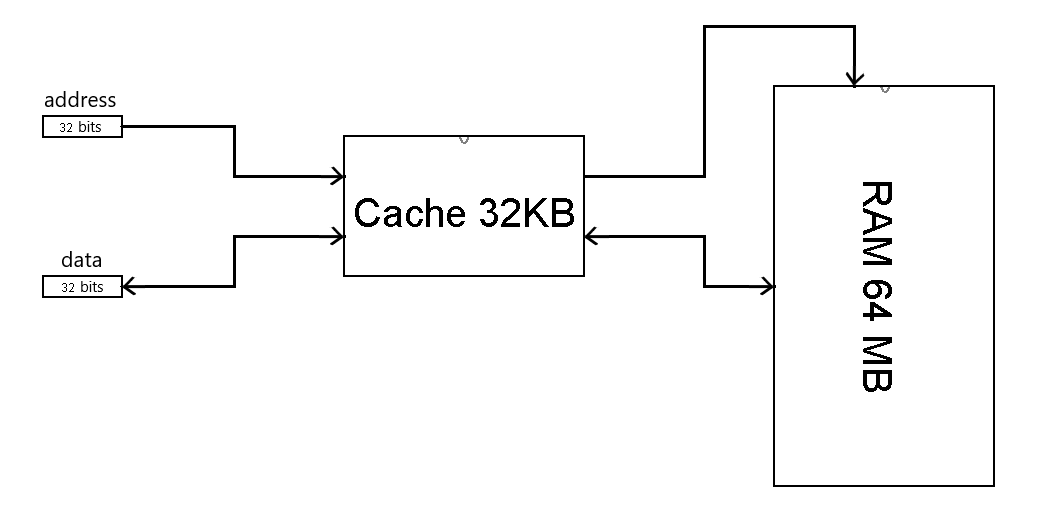
\includegraphics[width=\textwidth]{img.png}

We saw broadly in class how a memory cache works, but in this project we will dive to the detailed internals working of this technology, and almost all of the main parts and concepts are well described in the book "Digital Design and Computer Architecture, 2\textsuperscript{nd} edition" from the author \textit{David Harris}. You will find the essential materials in chapter 8 (\textit{8.3. Caches} pages 480-491). This project should be implemented using Logisim. Be warned, this project is not easy.

\newpage

\section{Guideline}

\begin{itemize}

    \item The cache is of type 2-ways set associative, with write-back write policy and LRU (Least Recently Used) replacement policy.
    \item For sake of simplicity, the cache and the main memory can only handle 32 bits words, even though the addressable cell is of 8 bit. The memories are realigned in 4 Bytes.
    \item Logisim can not handle the simultaneous input/output ports, which restricts the implementation to use 2 different ports, one for inputs and one for outputs.
    \item The response time of the cache is 1 cycle if the request hits, and many cycles otherwise. The read and write time of the main memory (RAM) is 10 cycles for one 32 bits word. You need to find the way to simulate that in Logisim.
    \item To overcome the synchronization problem caused by the differences in response time, we have to use a simple well known synchronization protocol. If a component wants to request a job from another, like CPU requesting data from the cache, a command line of the name of $request$ is used to inform the cache that CPU requests a data. The cache can take many cycles in the case of a "miss". Thus, a second command line is returned from the cache to the CPU called $Ready/\overline{Busy}$ informing the CPU when the cache finishes its processing and can retrieve the result. The same should be done for the cache interacting with the RAM.
    \item The use of external libraries is prohibited, while it is still allowed to use the internal libraries for components like, registers, counters, comparators...etc.
        
\end{itemize}

\section{Clauses and conditions}

\begin{itemize}

    \item The circuit should be done in one Logisim file and saved like \emph{.circ} file. The file should be sent to my email : \underline{Kara.Abdelaziz@el-kalam.com} with the student information.
    \item The dead end for submission is for 15/01/2024 at 00:00. The solution will be exposed just after.
    \item Only the first five valid submissions will be accepted, the sixth and after are not awarded.
    \item Completing the mini-project grants you a bonus score of 15 additional points to your TP grade.
    \item The project is intended to be done by one student, it is not a groupe project.
    \item The project to be accepted, needs to follow exactly the description and the terms of the guideline above.
    
\end{itemize}

\hspace*{\fill} \RL{وفقكم الله}

\end{document}